\documentclass[aps,twocolumn,pre]{revtex4-2}


\usepackage[utf8]{inputenc}
\usepackage{graphicx}
\usepackage{xcolor}
\usepackage{soul}
\usepackage{mathtools}
\newcommand{\red}{\textcolor{red}}


\usepackage[mathlines]{lineno}
\usepackage[normalem]{ulem}
\usepackage{lipsum}
%\usepackage{blindtext}
 \usepackage{amssymb,amsthm,amsmath} 

\newcommand{\kari}[1]{\textcolor{red}{#1}}
  
\begin{document}

 
\title{Influence of conspecific attraction on the distribution patterns of colonial bird nests} 

\author{Luciano C. López Bertazza$^{1}$}
\author{Karina Laneri$^{1,2}$}

\affiliation{$^{1}$ Statistical and Interdisciplinary Physics Division, Centro Atómico Bariloche (CNEA), R8402AGP Bariloche, Argentina}
\affiliation{$^{2}$ CONICET and Instituto Balseiro, Bariloche, Argentina}

\begin{abstract}

In nature, some birds forms colonies which don't have a characteristic size, this is specially common in species which don't have to fight for resource and the only force that play a role in the dynamic of the development of the lattice is an attractive one. In this job, we worked with a conspecific interaction which is stronger with the closeness of a nearby nest. We simulated this in a square periodic lattice and with an interaction between neighbour in a Moore vicinity of different ranges 1, 3 and 10. With the map provided by the simulation, we made analysis for the growing of one isolated colony and also for multiple colonies in the same lattice that can interact one with another. For the growing of the isolated colony we observed that for the bigger ranges the colony expanded quickly over the map and in a moment the arriving birds preferred to make a nest in the centre of the colony, therefore compacting the middle of it. This behaviour produced a variation in the fractal dimension, which started around $1.90(3)$ for the biggest visual range and increased with the addition of new birds until reaching the same value of the compacted clusters. We also searched for the dependency of the mean distance to the centre mass of the colony obtaining a power law with an exponent $z = 0{,}51(3)$, $z = 0{,}45(3)$ y $z = 0{,}39(3)$ for the different visual ranges analysed from lower to higher. Another power law dependency found was the relation between the area of the smaller convex polygon that contained every bird of the colony, resulting in an exponent equal to $0{,}97(3)$, $0{,}89(3)$ y $0{,}73(3)$ for visual ranges 1, 3 and 10. From this last results a mathematical equation was developed in order to measure the same exponent in the case of multiple colonies in the same map which can merge one with the other. This last analysis was only made for a visual range of 1 obtaining values that differed with the one obtained in the simulation of one colony and that its value depends on the value of the base probability to form new colonies, those values were $0.73(4)$ and $0.80(5)$ for the probabilities $10^{-5}$ and $10^{-7}$ respectively. Although the difference in the values, we were able to observe the power law behaviour in both simulations, ensuring that this behaviour provide no characteristic size of colonies.

\end{abstract}

\maketitle
 
\section{Introduction}

In nature, birds could be classified by their behaviour with animals of the same species (conspecific relation). At the extremes of this classification could be found on one side, territorial birds like the golden eagle (\textit{Aquila chrysaetos}), that defend its nest and its surroundings for lengths of the order of kilometres \cite{slater2017}. On the other side, colonials birds could be found as the white storks (\textit{Ciconia ciconia}) that prefer to nest near birds of the same species \cite{jovani2007}. In between of these two extremes, species with mixed behaviour could be found, such as the lesser kestrel \cite{jovani2008}, which is the most general conduct. With the mixed habits, the colonies show a characteristic size which can be explained, for example, by social interactions or by the heterogeneity of the terrain. In contrast to this, birds that present extreme colonial behaviour as the Audouin's gull (\textit{Larus adouinii}) or the white stork (\textit{Ciconia ciconia}) \cite{jovani2007}, a fractal spatial distribution of nests could be found, showing nests of all sizes and therefore putting in check the concept of a characteristic colony size commonly accepted in ecology. One of the hypothesis that could explain the free scale colony behaviour is the conspecific attraction, which has been found to be key for the growing colonies of some maritime birds \cite{tenan2017}.

In this work, a spatially explicit and probabilistic model was proposed, inspired in \cite{tesis2006} Chap.7, which uses the conspecific attraction to replicate the behaviour of nesting of colony birds. The model has been expanded and implemented in numerical simulations, exploring how the density of birds and their visual range of interaction affect the morphology and spatial distribution of the colony of nests.

Given that in many species it is difficult to experimentally isolate the factors that influence the spatial distribution of nests, the usage of computational models allows the exploration of controlled sceneries, with a systematic variation of the parameters of the model \cite{bascompte1995, stauffer1994}. 

\section{Simulation Model}
\label{Modelo}

The simulation runs in a two-dimensional lattice of size $L \times L$ conformed by discrete spaces. In this map, nest are aleatory added $n$ as seed nests. After this, the simulation continues by selecting a random place of the grid and decides whether to add a new nest or not, by following the Social Context (CS) function, which is defined as:

\begin{equation*}
    SC = \frac{1}{C} \sum_{i=1}^{n} \left( \frac{N_{\text{neigh}}(i)}{N_{\text{sites}}(i)} \cdot \frac{1}{i} \right)
\end{equation*}

in this equation:
\begin{itemize}
\item $C$ is a normalization constant that follows: $C = \sum_{i=1}^{n} \frac{1}{i}$

\item $N_{\text{sites}}(i) = 8i$ represents the number of sites which are in the Moore neighbourhood of range $i$

\item $N_{\text{neigh}}(i)$ is the number of nests that are inside the neighbour

\item $n$ is the maximum distance of interaction between birds, which is called the \textit{visual range}.
\end{itemize}
\vspace{0.5em}

The following section describes the functionality of the simulation. For further details, the codes are available in ~\cite{Lucho_codigos}, which are coded in Python as well as in C++.


\vspace{1em}

1. \textbf{initialization of the map}: a square lattice is created of length $L \times L$, where every spot begins as a zero, meaning that is unoccupied, in which $L$ is a power of two. 

2. \textbf{aggregation of seed nest}: a $5\%$ of the total birds are added with a random distribution on the map avoiding occupied spaces, if another nest is in the randomly selected tile the seed bird try again selecting another random tile until selects a free one.

3. \textbf{aggregation of the rest of birds}: Once the seed birds are added, the simulation continues by adding the rest of birds one by one. In each time, the bird selects a random place on the grid and has a probability of forming a nest equal to the equation of social context calculated on that site. In the case that no nest is inside the visual range of the bird, a base probability was added to the code in order to speed up the simulation. In most of the analysis, this probability is $P_{base}=1 \times 10^{-7}$.

4. \textbf{Selection of the total number of birds}: this parameter is fixed by the selection of the density of the population of birds.

\vspace{1em}

The code of this simulation was started in Python to then be converted to C++, in order to reduce the running time. The simulations were run on the "Cluster de Computos de CPU de la Gerencia de Física del CAB". All results presented were obtained by averaging 10 simulation runs with the same parameters.

\section{Results}
\subsection{Simulation of only one colony}
\subsubsection{Study of the mass in function of the distance}

One of the available methods to calculate the fractal dimension is through studying the number of nests (also called mass) that are contained in a circle of radius R, further explanation can be found in \cite{Fractales_libro}. 

In order to do such analysis, the simulation calculates the distance to the centre of the cluster of each nest and then show how many of those are within a radius of R. The number of nest has a power law dependency with the radius in which the power is called the fractal dimension ($d_f$), shown below:

\begin{equation}
    N \approx R^ {d_f} 
\label{dimfac}    
\end{equation}

With this in mind, is possible to obtain the value of the $d_f$ by plotting N as a function of R in log-log scale and then fitting a lineal function, in which the slope is the fractal dimension. In cases where the slope has a value of 1, it means that the cluster grows at a linear scale. Meanwhile, a value of 2 indicates a compact growth in a two-dimensional space. Therefore, in fractal patterns the value of $d_f$ must be between the numbers previously talked about


The previously explained method was used to study the growth of an only cluster, which seed nest was allocated in the middle of the grid. The rest of the nests followed the $SC$ function with visual ranges 1, 3 and 10. The results were compared with a circle and a square cluster, which are shown in the plot \ref{A(r)}.


\begin{figure}[h!]
    \centering
    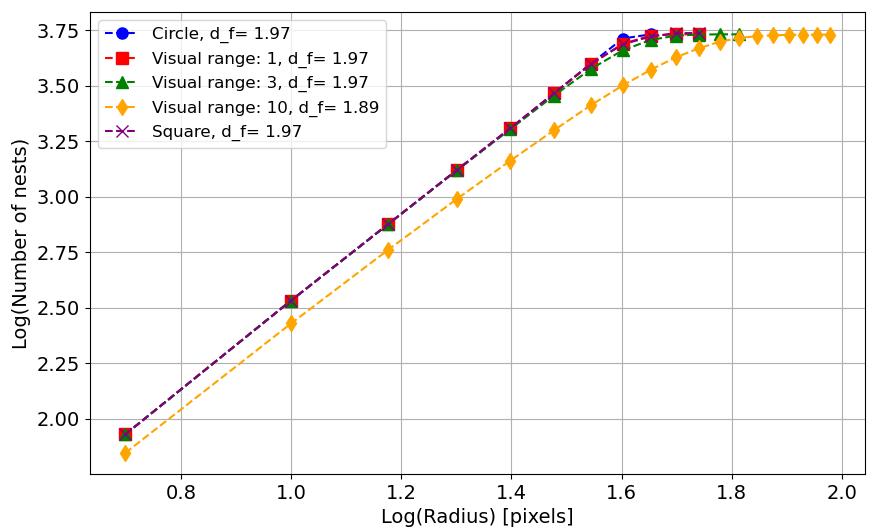
\includegraphics[width=0.95\linewidth]{Figuras/N_r.png}
    \caption{Dependency of the number of nests with the radius to the centre of the cluster.}
    \label{A(r)}
\end{figure}

It can be observed that the simulation with a visual range of 10  have a fractal dimension lower than all the other. While the rest of the simulations have a $d_f=1.97(3)$, the one with the highest vision have a slope of $1.89(3)$. To understand this results, in the Fig. \ref{1cluster} the structure of the different distributions are shown.

\begin{figure}[h!]
    \centering
    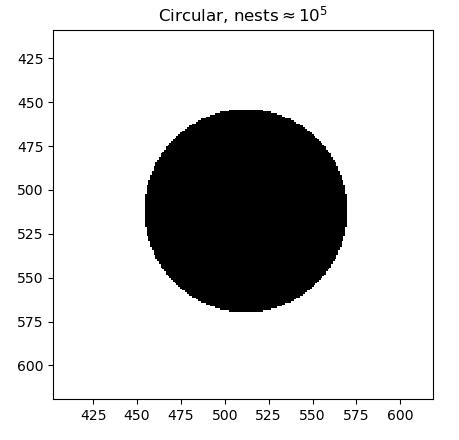
\includegraphics[width=0.48\linewidth]{Figuras/Circular distribution.png}
    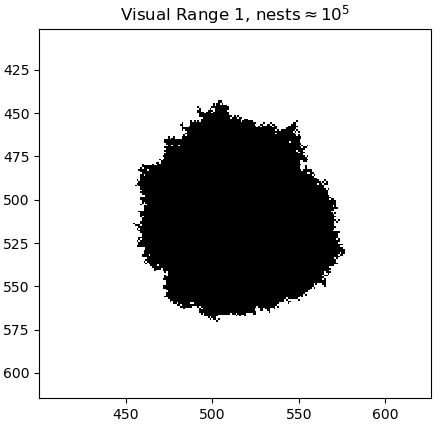
\includegraphics[width=0.48\linewidth]{Figuras/VR1 distribution.png}
    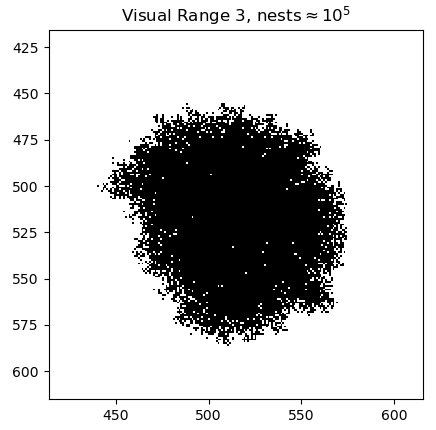
\includegraphics[width=0.48\linewidth]{Figuras/VR3 distribution.png}
    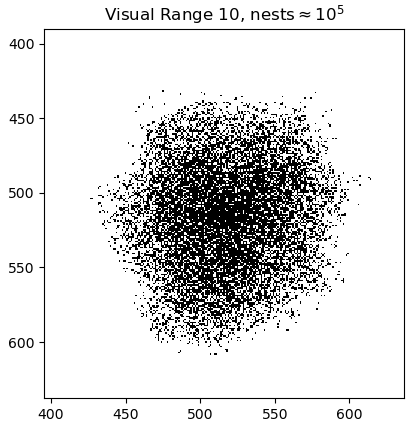
\includegraphics[width=0.48\linewidth]{Figuras/VR10 distribution.png}
    \caption{Examples of clusters for the deferents distributions of nests.}
    \label{1cluster}
\end{figure}

Since the linear fitting needs to be done on the medium range of the curve, as is where the curve shows this behaviour, the analysis doesn't take in to consideration the borders of the cluster. Because of this, the clusters with lower visual range present a similar visual range as the circular distribution, as they are compacted in the interior. In the figure \ref{A(r)}, the curve of visual range 3 is slightly lower, and this is because of the few spaces left unoccupied by the birds, making the cluster not completely compacted. Following this tendency, the distribution of the one with a visual range of 10 presents more free spaces, making slope even lower.

In this model, the dynamics of conspecific attraction cause the distributions to become increasingly concentrated toward the centre as the number of nests increases. As a consequence of this, the variation of the fractal dimension with the number of birds was study, which can be found in the Appendix (\ref{d_f N(r)}). This analysis show a stable $d_f$ for small colonies up until the moment when the arriving birds start to prioritize nesting in the centre of the colony rather than in its borders. Therefore, the new nest start to saturate the centre of the cluster, making it more compact and with a fractal dimension more near the one of the circular distribution.


\subsubsection{Evolution of the length of the cluster with time}

The growing of only one cluster was simulated for the visual ranges 1, 3 and 10. During this process, every few nests the code would calculate the centre of mass(${\bf x}_{cm}$) of the colony in order to later get its characteristic length $L(t)$, which follows the next equation
\begin{equation*}
    L(t) \approx \sqrt{\sum_{i=0}^{N-1} ({\bf x}_i - {\bf x}_{cm})^2/N} \, 
\end{equation*}

 This process is repeated 10 times for each set of variables, in order to reduce the statistic noise. In Fig. \ref{Exponente dinamico}, the characteristic length is plotted as a function of the number of nests.

\begin{figure}[h!]
    \centering
    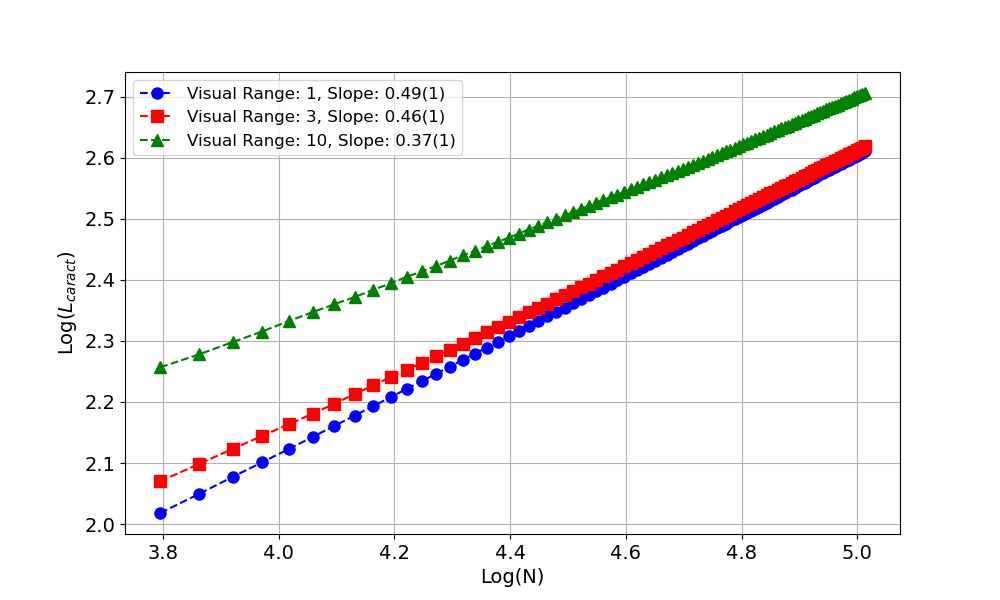
\includegraphics[width=0.95\linewidth]{Figuras/L(N).png}
    \caption{Graphic of the dependency of ($L_{caract}$) with the number of nests}
    \label{Exponente dinamico}
\end{figure}

The graph shows a power law dependency between the characteristic length and the number of nests. This dependency is described by the following equation:
\begin{equation}
\langle L(N) \rangle \sim N^{1/z}
\end{equation}

where $N$ is the number of nests, $\langle L \rangle$ is the length of the colony, and $z$ is the dynamic exponent. This exponent shows a tendency to decrease its value as the visual range is incremented. This can be explained by the possibility of the birds to nest at a greater distance as the visual range increases, which allows a quick expansion of the colony. Therefore, in order to reach the same length of the colony, fewer birds are needed for the simulations with greater visual ranges.


\subsubsection{Dependency of the area with the number of birds}
Another property analysed was the area of the Convex Hull and its relation with the number of nests. The value of this area is obtained by using a function of the library \textit{scipy.spatial}, which receive a vector of coordinates and make the smallest polygon with the furthermost points and then can return the area of said polygon or its perimeter. The Fig. \ref{C_Hull} shows the dependency of this area with the number of nests for the different visual ranges.


\begin{figure}[h!]
    \centering
    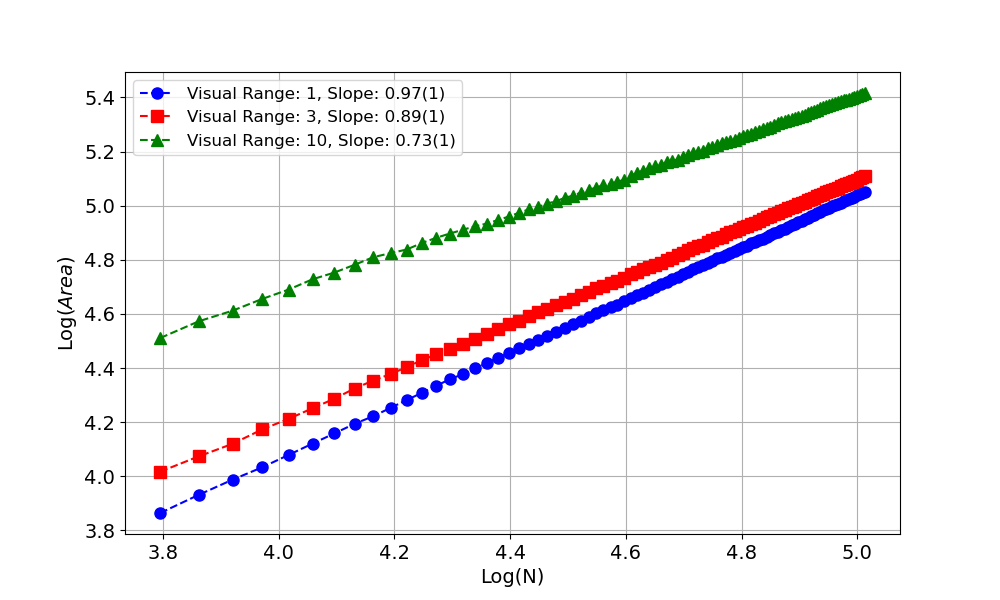
\includegraphics[width=0.95\linewidth]{Figuras/A(n).png}
    \caption{Graphic of the dependency of area of the \textit{Convex Hull} with the number of nests.}
    \label{C_Hull}
\end{figure}

It can be observed how this curves follow a power law behaviour between the area of the convex hull and the number of birds($N$), resulting in the following equation

\begin{equation}
\langle S(N) \rangle \sim N^{\beta}
\label{areamasa}
\end{equation}

where  $\langle S \rangle$ is the average area of the convex hull and $\beta$ is the exponent of the power law. The plot also shows how this exponent because smaller with the increase of the visual range, this can be explained by the variation of compactness of the cluster. As the simulation with visual ranges bigger than 1 grow leaving some spaces between nests, their area increase quickly at the beginning, but at a certain moment the centre of the cluster become suitable for nesting and therefore birds starts to allocate there. This birds that form a nest in the centre of the colony do not increase the area of the cluster. As a consequence, the growth of the area slows and reduce the value of $\beta$.

Because in this model, the evolution of time is proportional to the adding of nests, the equation above can be written as follows:
\begin{equation}
\langle S(t) \rangle \sim t^{\beta}
\label{areatiempo}
\end{equation}
This expression will be used in the following section


\subsection{Distribution of sizes of colonies}

\subsubsection{Analytical development}
Given the results obtained for one and multiple colonies, an analytical expression was developed to understand the origin of the power laws found in different scales.



Because of eq.~\ref{dimfac}, it has been shown that:
\begin{equation*}
    N \approx R^ {d_f} 
\end{equation*}
Also, using eq.~\ref{areamasa}, we have:
\begin{equation*}
\langle S(N) \rangle \sim N^{\beta}
\end{equation*}
Furthermore, from eq.~\ref{areatiempo} we obtain, for a single colony:
\begin{equation*}
\langle S(t) \rangle \sim t^{\beta}
\end{equation*}


Thus, being $S_i(t)$ the area of the colony $i$ at the time $t$ and using the equations above, the subsequent formula can be written:

\begin{equation*}
\langle S_i(t) \rangle \approx \alpha (t-t_i)^\beta     \, ,
\end{equation*}

in which $t_i$ is the time where the colony $i$ was formed.

Having into consideration that the colonies start at different moments, the distribution of sizes of colonies for a certain moment of the simulation can be written as:

\begin{equation*}
    P(S,t) = \int_0^t \rho(t_i) \delta(S-S_i(t)) dt_i
\end{equation*}

where $\rho (t)$ is the nucleation probability density at a time $t$. By using the mathematical property where $\delta(f(x))=\delta(x-x_0)/|f'(x_0)|$, for every function $f(x)$ which has only one zero ($f(x_0)=0$), the equation can be rewritten as:

\begin{equation*}
    P(S,t) = \frac{\rho(t-(S/\alpha)^{1/\beta})}{\alpha \beta (S/\alpha)^{(\beta-1)/\beta}} \sim S^{-(\beta-1)/\beta}
\label{tamaniosclusters}
\end{equation*}

in which the last approximation comes from taking the nucleation probability density as a constant in time. This condition is most certainly true for the beginning of the simulation. Nevertheless, with the passing of time $\rho$ decreases, given that the new birds would form a nest with greater probability inside a colony already formed.


\subsubsection{Simulations}
In order to corroborate this analytic development with the distribution of sizes of clusters obtained in the simulations, the system was let to evolve until a certain moment where the colonies were counted and their sizes measured. The criteria used to define a colony were that if two nest are at a distance lower to the visual range, then they are from the same colony. With the data collected, a plot was made with the frequency of appearance in function of the colony size for different sizes of maps, different base probability of forming nest and only for visual range of 1, this plot is show in the Fig. \ref{freq}.

\begin{figure}[h!]
    \centering
    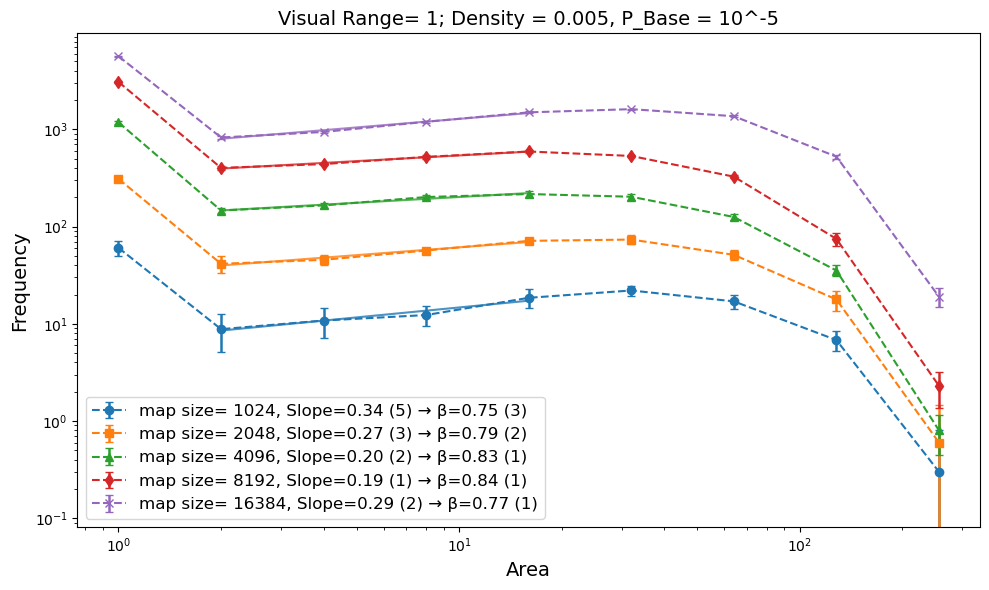
\includegraphics[width=0.95\linewidth]{Figuras/Frequency P_base-5.png}
    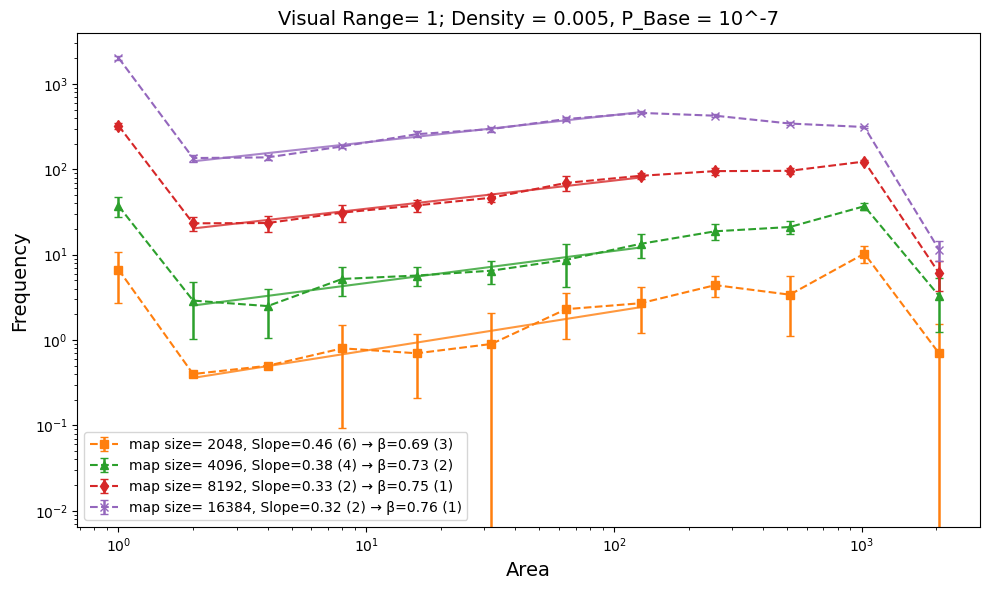
\includegraphics[width=0.95\linewidth]{Figuras/Frequency P_base-7.png}
    \caption{Plots for the frequency of appearances for the different sizes of colonies, for different size of maps and distinct base probability of forming a nest.}
    \label{freq}
\end{figure}

With a higher base probability of forming a nest, the number of small colonies increase at the expense of the bigger colonies, which produce smoother curves. Also, with the increase of the base probability, the value of $\beta$ increases slightly, for $P_{Base}=10^{-7}$ $\xrightarrow{}$ $\beta \approx 0.73(4)$ and for $P_{Base}=10^{-5}$ $\xrightarrow{}$ $\beta \approx 0.80(5)$. Another observation is that, with probabilities, with the increase of the map the grater is the value of $\beta$, except for the biggest map of the bigger base probability. It is important to remark that all the values obtained for $\beta$ differ with the one from the single colony simulation, further analysis is needed to explain it, but it is probable that cause is in the supposition of a fixed value for the nucleation probability density.


\section{Conclusions}

In this job, spatial simulations were used in order to recreate the spatial distribution of colonial birds by proposing only an attractive interaction, such as the conspecific interaction present in nature. The mathematical model added as a consideration the range of interaction, making it a parameter of the simulation.

In the simulations of a single colony, a power law dependency was found between the number of nests and the radius of the cluster. The exponent of this tendency increase with augment of the number of nest in the colony until it saturates at a value of 2 and decreases for higher visual ranges.

The same functionality was found in the evolution of the characteristic length and the area of the convex hull of one colony with the aggregation of nests. In the first case the exponents obtained were $z=0.49(1)$, $z=0.46(1)$ y $z=0.37(1)$ for visual ranges 1,3 and 10 respectably. While in the second, the values were $\beta=0.97(1)$, $\beta=0.89(1)$ y $\beta=0.73(1)$ for the same visual ranges


In the simulation of multiple colonies with a visual range of 1, the frequency of appearance of colonies of a certain area with logarithmic bins of base 2 shows a power law tendency for the medium size clusters. A mathematical expression was achieved in order to relate the exponent of the multiple colonies simulation with the exponent of the area of the convex hull of one colony. The value of $\beta$ obtained with the mathematical equation change with the value of the parameter of base probability to form a new colony, obtaining $\beta=0.73(4)$ for $P_{Base}=10^{-7}$ and $\beta=0.80(5)$ for $P_{Base}=10^{-5}$.

Further work is needed to explain the discrepancy of the values of $\beta$ between the simulation of multiple colonies and the one of a single colony. Adding the effects of a non-fixed value for the nucleation probability density to the equation is heavily encouraged.




\bibliography{bibaves}



\onecolumngrid

\newpage
\appendix

\renewcommand{\thefigure}{a\arabic{figure}}
\renewcommand{\thesubsection}{A\arabic{subsection}}
\setcounter {figure} {0}

\subsection{Fractal dimension for different number of nests}
\label{d_f N(r)}

With the increase of the density of birds, and therefore the increase in nest, the simulation with visual range of 10 approach the fractal dimension of the square simulation, as shown in the Figure \ref{Problema Nro de aves}


\begin{figure}[h!]
    \centering 
    
\includegraphics[width=0.45\linewidth]{Appendix/A(r) low density.png}
    
\includegraphics[width=0.45\linewidth]{Appendix/A(r) high density.png}
    \caption{Analysis of the dependency of the number of nest with the distance to the centre of the colony.}
    \label{Problema Nro de aves}
\end{figure}
As a consequence of these discrepancies between the fractal dimensions, a study of the same analysis for different number of nests. The results of this is shown in the Figure \ref{D_frac_vs_N}.

\begin{figure}[h!]
    \centering
    
\includegraphics[width=0.5\linewidth]{Appendix/Fractal dimension vs number of nests.png}
    \caption{Fractal dimension of one cluster in function of the nests it contains.}
    \label{D_frac_vs_N}
\end{figure}

It is necessary to clarify that the reason why the compacted systems differ from the expected value of two, can be explained by taking in to consideration the discrete properties of the map, while it was designed for a continuos space. Another observable result is the stable fractal dimension of $1.90(3)$ for a low number of nests for the visual range of 10. When this stability breaks, the value of $d_f$ increases until reaching the one of the compacted distributions. To better understand this result on Figure \ref{Problema Nro de aves clusteres} examples of the simulations are shown for the different visual ranges and number of birds.


\begin{figure}[h!]
    \centering
    
\includegraphics[width=0.25\linewidth]{Appendix/1col lowest dens.png}
    
\includegraphics[width=0.25\linewidth]{Appendix/1col 2nd dens.png}\\
    
\includegraphics[width=0.25\linewidth]{Appendix/1col 3rd dens.png}
    
\includegraphics[width=0.25\linewidth]{Appendix/1col highest dens.png}
    \caption{Maps for the simulation with a visual range of 10, for different number of nest in a map of 1024x1024}
    \label{Problema Nro de aves clusteres}
\end{figure}

These maps show how the increase in number of nests make the centre more compact, which could explain the increase in the fractal dimension.

\subsection{Maps for different numbers of nests and different visual}

\begin{figure}[h!]
    \centering
    
\includegraphics[width=0.3\linewidth]{Appendix/Map 0.001 1.png}
    
\includegraphics[width=0.3\linewidth]{Appendix/Map 0.001 3.png}
    
\includegraphics[width=0.3\linewidth]{Appendix/Map 0.001 10.png}
    
\includegraphics[width=0.3\linewidth]{Appendix/Map 0.01 1.png}
    
\includegraphics[width=0.3\linewidth]{Appendix/Map 0.01 3.png}
    
\includegraphics[width=0.3\linewidth]{Appendix/Map 0.01 10.png}
    \caption{Example of the maps obtained for the different configurations of visual range and density of birds.}
    \label{Mapas densidades y rangos}
\end{figure}



 




\end{document}
